% Figure consists of 4 parts (in this order in the code)
% Surface D (upper left)
% Detail plot highlighted square (lower left)
% Surface S (non-linear transformation of surface D) (upper right)
% Detail plot highlighted square on surface S (lower right)
\documentclass{article}
\usepackage{tikz}
\usepackage{float}
\usepackage{lmodern}
\usepackage{amsmath}
\usetikzlibrary{calc}
\usetikzlibrary{decorations.markings}
\usetikzlibrary{arrows, arrows.meta}
\usetikzlibrary{patterns,patterns.meta}
\usepgfmodule{nonlineartransformations}

\begin{document}

\centering

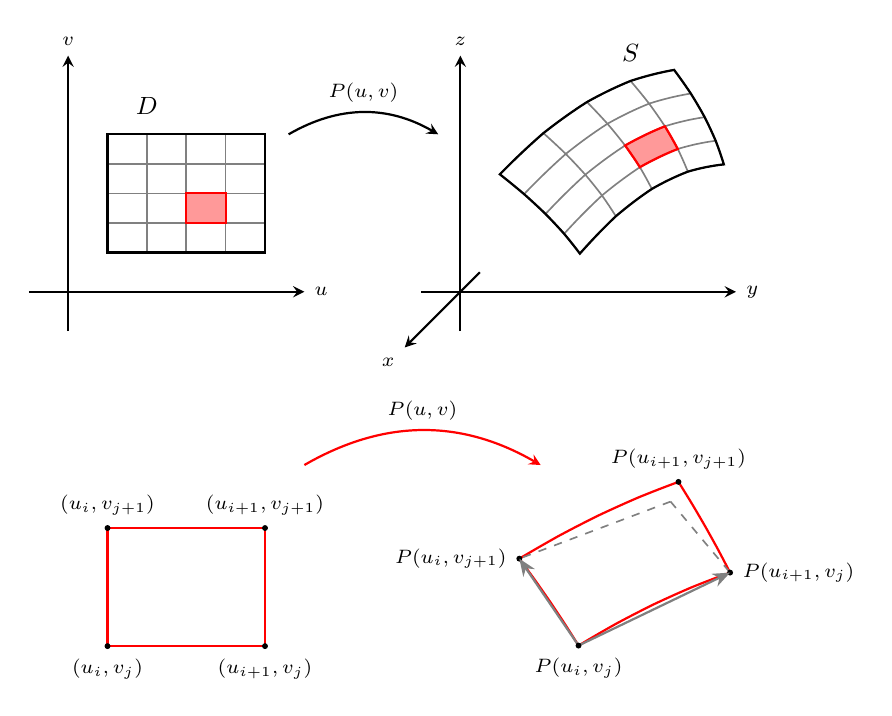
\begin{tikzpicture}[scale=1.0]  % set scale same as picturescale!
\pgfmathsetmacro{\PictureScale}{1.0}
\pgfmathsetmacro{\CircleSize}{0.03}     % radius of coordinate circles/dots
% conversion from cm to pt and vice versa
\pgfmathsetmacro{\CmToPt}{28.3464566929}
\pgfmathsetmacro{\PtToCm}{0.0352777778}
% define styles used in this picture
\tikzset{every node/.style={font=\scriptsize,text=black},
CircleNodeStyle/.style={draw=black, shape=circle, fill=black, minimum size=\CircleSize*2 cm, inner sep=0pt},
arrowstyle/.style={->, >=stealth}}

% first axis
\pgfmathsetmacro{\OvershootAxis}{0.5} 
\draw[arrowstyle, thick] (-\OvershootAxis,0) -- (3,0) node[pos=1, right] {$u$};
\draw[arrowstyle, thick] (0,-\OvershootAxis) -- (0,3) node[pos=1, above] {$v$};

% second axis
\pgfmathsetmacro{\OvershootAxis}{0.5}
\pgfmathsetmacro{\SecondAxisOffset}{5}  % xshift for second axis
\begin{scope}[xshift=\SecondAxisOffset * \CmToPt]
    % x and z-axes
    \draw[arrowstyle, thick] (-\OvershootAxis,0) -- (3.5,0) node[pos=1, right] {$y$};
    \draw[arrowstyle, thick] (0,-\OvershootAxis) -- (0,3.0) node[pos=1, above] {$z$};
    % y-axis (angled)
    \pgfmathsetmacro{\ZAxisBeginX}{cos(45) * \OvershootAxis * 0.7}
    \pgfmathsetmacro{\ZAxisBeginY}{ sin(45) * \OvershootAxis * 0.7}
    \pgfmathsetmacro{\ZAxisEndX}{- cos(45)*1.0}
    \pgfmathsetmacro{\ZAxisEndY}{ - sin(45) * 1.0}
    \draw[arrowstyle, thick] (\ZAxisBeginX, \ZAxisBeginY) -- (\ZAxisEndX, \ZAxisEndY) node[pos=1, below left] {$x$};
\end{scope}

% surface D (u and v)
\pgfmathsetmacro{\Startuv}{0.5}
\pgfmathsetmacro{\Endu}{2.5}
\pgfmathsetmacro{\Endv}{2}
\pgfmathsetmacro{\usegments}{4}
\pgfmathsetmacro{\vsegments}{4}
\pgfmathsetmacro{\ustepsize}{(\Endu-\Startuv)/\usegments}
\pgfmathsetmacro{\vstepsize}{(\Endv-\Startuv)/\vsegments}

% u and v index, of highlighted rectangle
\pgfmathsetmacro{\HiglightedIndexU}{3}
\pgfmathsetmacro{\HiglightedIndexV}{2}

% draw the surface D segments
\foreach \uindex in {0,...,\usegments}
    \pgfmathsetmacro{\ucoord}{\Startuv + \ustepsize * \uindex}
    \draw[semithick, gray] (\ucoord, \Startuv) -- (\ucoord, \Endv);
\foreach \vindex in {0,...,\vsegments}
    \pgfmathsetmacro{\vcoord}{\Startuv + \vstepsize * \vindex}
    \draw[semithick, gray] (\Startuv, \vcoord)--(\Endu,\vcoord);
% draw contour of surface D and add node
\draw[thick, black]  (\Startuv, \Startuv) -- (\Endu, \Startuv) -- (\Endu, \Endv) -- (\Startuv, \Endv) -- cycle;
\node [label=above:\small{$D$}] at (\Startuv + \ustepsize, \Endv) {};

% Detail plot highlighted square
% define corners of highlighted square and draw highlighted square
\pgfmathsetmacro{\HighlightedMinU}{\Startuv + (\HiglightedIndexU - 1.0) * \ustepsize}
\pgfmathsetmacro{\HighlightedMaxU}{\Startuv + (\HiglightedIndexU) * \ustepsize}
\pgfmathsetmacro{\HighlightedMinV}{\Startuv + (\HiglightedIndexV - 1.0) * \vstepsize}
\pgfmathsetmacro{\HighlightedMaxV}{\Startuv + (\HiglightedIndexV) * \vstepsize}
\draw[thick, red, postaction={fill=red, opacity=.4}] (\HighlightedMinU, \HighlightedMinV) -- (\HighlightedMaxU, \HighlightedMinV) -- (\HighlightedMaxU, \HighlightedMaxV) -- (\HighlightedMinU, \HighlightedMaxV) -- cycle;

% define detail of highlighted square
\pgfmathsetmacro{\ScaleHighlightDetailPlot}{4}      % scale factor of the detail plot
\pgfmathsetmacro{\XShift}{-\HighlightedMinU * \ScaleHighlightDetailPlot + \Startuv}
\pgfmathsetmacro{\YShift}{-\HighlightedMinV * \ScaleHighlightDetailPlot - 4.5}
\coordinate (Shift) at (\XShift, \YShift);
% draw detail of highlighted square
\begin{scope}[shift={(Shift)}, scale=\ScaleHighlightDetailPlot]
    \draw[thick, red] (\HighlightedMinU, \HighlightedMinV) -- (\HighlightedMaxU, \HighlightedMinV) -- (\HighlightedMaxU, \HighlightedMaxV) -- (\HighlightedMinU, \HighlightedMaxV) -- cycle;
    \node [CircleNodeStyle, label=below:{$(u_{i}, v_{j})$}] at (\HighlightedMinU, \HighlightedMinV) {};
    \node [CircleNodeStyle, label=below:{$(u_{i+1}, v_{j})$}] at (\HighlightedMaxU, \HighlightedMinV) {};
    \node [CircleNodeStyle, label=above:{$(u_{i+1}, v_{j+1})$}] at (\HighlightedMaxU, \HighlightedMaxV) {};
    \node [CircleNodeStyle, label=above:{$(u_{i}, v_{j+1})$}] at (\HighlightedMinU, \HighlightedMaxV) {};
\end{scope}

% surface S (non-linear transformation of surface D)
% the nonlinear transformation is calibrated on a certain figure
% dimensions of calibrated surface
\pgfmathsetmacro{\XWidthOrig}{7.0}
\pgfmathsetmacro{\YWidthOrig}{7.0}
\pgfmathsetmacro{\StartXOrig}{0.0}
\pgfmathsetmacro{\StartYOrig}{5.0}
% nonlinear parts of the transformation (x^2, x*y...) need to be scaled to calibration size (via "scale") to ensure no deformation (non-linear transformation on figure size 10 won't have same effect as on a figure with size 1)
\pgfmathsetmacro{\Xscale}{(\Endu - \Startuv) / (\XWidthOrig*1.4)}   % original object xdim / calibrated object xdim
\pgfmathsetmacro{\Yscale}{(\Endv - \Startuv) / (\YWidthOrig*1.4)}
\pgfmathsetmacro{\scale}{(\Xscale+\Yscale)/2 * \PictureScale}
\pgfmathsetmacro{\ScopeScale}{0.8}                      % applied zoom-factor (in scope)
\pgfmathsetmacro{\ScaleInScope}{\ScopeScale * \scale}   % resulting scale in scope

% Function: non linear transformation
% nonlinear parts (x^2, x*y, ...) were selected by adding them one by one for desired result
\makeatletter
\def\CustomNonlinearTransformation#1#2#3{%
% #1: x shift
% #2: y shift
% #3: scaling factor
\pgfmathsetmacro{\offsetx}{\pgf@x + #1}
\pgfmathsetmacro{\offsety}{\pgf@y + #2}
\pgfmathsetmacro{\myX}{\offsetx - 0.001*\pgf@y*\pgf@y / #3 + 0.001*\pgf@x*\pgf@y / #3} %
\pgfmathsetmacro{\myY}{\offsety - 0.002*\pgf@x*\pgf@x / #3 + 0.0005*\pgf@x*\pgf@y / #3} %
\setlength{\pgf@x}{\myX pt}
\setlength{\pgf@y}{\myY pt}
}
\makeatother

% define corners of transformation highlighted square: flip indices for X as image appears to be flipped
\pgfmathsetmacro{\ScaledXOrig}{\StartXOrig * \scale}
\pgfmathsetmacro{\ScaledYOrig}{\StartYOrig * \scale}
\pgfmathsetmacro{\MaxX}{\ScaledXOrig - \ustepsize * (\usegments)}
\pgfmathsetmacro{\MaxY}{\ScaledYOrig + \vstepsize * (\vsegments)}

% track the position of non-linear transformation with no shift. Resulting position of the tracker is then used to position figure
\def\TrackPosition#1#2#3#4{%
%#1: Tracker x-position
%#2: Tracker y-position
%#3: ScopeScale
%#4: ScaleInScope
\begin{scope}[scale=#3]
    \pgftransformnonlinear{\CustomNonlinearTransformation{0.0}{0.0}{#4}}
    \coordinate (Tracker) at (#1, #2);
\end{scope}
% extract x- and y-dimension
\newdimen\xshiftneg 
\newdimen\yshiftneg
\pgfextractx{\xshiftneg}{\pgfpointanchor{Tracker}{center}} 
\pgfextracty{\yshiftneg}{\pgfpointanchor{Tracker}{center}}
% shift is the inverse of the tracker position
\pgfmathsetmacro{\xshiftOrig}{ -\xshiftneg} 
\pgfmathsetmacro{\yshiftOrig}{ -\yshiftneg}
}

% define x- and y-shift
\TrackPosition{\MaxX}{\MaxY}{\ScopeScale}{\ScaleInScope}
\pgfmathsetmacro{\xshiftTot}{\xshiftOrig + (\SecondAxisOffset + 0.5) * \CmToPt } 
\pgfmathsetmacro{\yshiftTot}{\yshiftOrig + 1.5*\CmToPt}

% define corners of transformation highlighted square: flip indices for X as image appears to be flipped
\pgfmathsetmacro{\HighlightedMinX}{- \ustepsize * (\usegments - \HiglightedIndexU + 1)}
\pgfmathsetmacro{\HighlightedMaxX}{- \ustepsize * (\usegments - \HiglightedIndexU)}
\pgfmathsetmacro{\HighlightedMinY}{ \vstepsize * (\HiglightedIndexV - 1)}
\pgfmathsetmacro{\HighlightedMaxY}{ \vstepsize * (\HiglightedIndexV)}

% draw surface D and apply non linear transformation -> surface S
\begin{scope}[scale=\ScopeScale, xshift=\ScaledXOrig * \CmToPt, yshift=\ScaledYOrig * \CmToPt, draw=gray]
    \pgftransformnonlinear{\CustomNonlinearTransformation{\xshiftTot *  \PictureScale}{\yshiftTot * \PictureScale}{\ScaleInScope}}
    % draw the surface S segments
    \foreach \uindex in {0,...,\usegments}
        \pgfmathsetmacro{\Xcoord}{- \ustepsize * \uindex}
        \pgfmathsetmacro{\YcoordA}{\vstepsize * \vsegments}
        \pgfmathsetmacro{\YcoordB}{0}
        \draw[semithick] (\Xcoord, \YcoordA)--(\Xcoord, \YcoordB);
    \foreach \vindex in {0,...,\vsegments}
        \pgfmathsetmacro{\Ycoord}{\vstepsize * \vindex}
        \pgfmathsetmacro{\XcoordA}{ - \ustepsize * \usegments}
        \pgfmathsetmacro{\XcoordB}{0}
        \draw[semithick] (\XcoordA, \Ycoord)--(\XcoordB, \Ycoord);
    % draw contour of surface D and highlighted square
    \draw[thick, black]  (0, 0) -- ( - \ustepsize * \usegments,  0) -- ( - \ustepsize * \usegments,  \vstepsize * \vsegments) -- (0, \vstepsize * \vsegments) -- cycle;
    \draw[thick, red, postaction={fill=red, opacity=.4}] (\HighlightedMinX, \HighlightedMinY) -- (\HighlightedMaxX, \HighlightedMinY) -- (\HighlightedMaxX, \HighlightedMaxY) -- (\HighlightedMinX, \HighlightedMaxY) -- cycle;
    \coordinate (SNodeCoord) at (- \ustepsize, \vstepsize * \vsegments);     % coord for S-node (nodes don't transform well direclty with nonlinear transformations...)
\end{scope}
\node [label=above:\small{$S$}] at (SNodeCoord) {};

% detail plot highlighted square on surface S 
% scale for detail plot
\pgfmathsetmacro{\ScopeScale}{\ScaleHighlightDetailPlot * \ScopeScale}
\pgfmathsetmacro{\ScaleInScope}{\ScopeScale * \scale}

% define x- and y-shift
\TrackPosition{\HighlightedMinX + \ScaledXOrig}{\HighlightedMinY + \ScaledYOrig}{\ScopeScale}{\ScaleInScope}
\pgfmathsetmacro{\xshiftTot}{\xshiftOrig + (\SecondAxisOffset + 1.5) * \CmToPt } 
\pgfmathsetmacro{\yshiftTot}{\yshiftOrig - 4.5*\CmToPt}

% draw highlighted square in surface S
\begin{scope}[scale=\ScopeScale, xshift=\ScaledXOrig * \CmToPt, yshift=\ScaledYOrig * \CmToPt]
    \pgftransformnonlinear{\CustomNonlinearTransformation{\xshiftTot * \PictureScale}{\yshiftTot * \PictureScale}{\ScaleInScope}}
    \coordinate (LowerLeft) at (\HighlightedMinX, \HighlightedMinY);
    \coordinate (LowerRight) at (\HighlightedMaxX, \HighlightedMinY);
    \coordinate (UpperRight) at (\HighlightedMaxX, \HighlightedMaxY);
    \coordinate (UpperLeft) at (\HighlightedMinX, \HighlightedMaxY);
    \draw[thick, red] (\HighlightedMinX, \HighlightedMinY) -- (\HighlightedMaxX, \HighlightedMinY) -- (\HighlightedMaxX, \HighlightedMaxY) -- (\HighlightedMinX, \HighlightedMaxY) -- cycle;
\end{scope}

\coordinate (UpperRightParallellogram) at ($(UpperRight)+(-0.10,-0.25)$);
\draw[semithick, gray, dashed] (UpperRightParallellogram) -- (LowerRight);
\draw[semithick, gray, dashed] (UpperRightParallellogram) -- (UpperLeft);
%\node [CircleNodeStyle, gray] at (UpperRightParallellogram) {};

\node [CircleNodeStyle, label=right:{$P(u_{i+1}, v_{j})$}] at (LowerRight) {};
\node [CircleNodeStyle, label=above:{$P(u_{i+1}, v_{j+1})$}] at (UpperRight) {};
\node [CircleNodeStyle, label=left:{$P(u_{i}, v_{j+1})$}] at (UpperLeft) {};

% arrows of parallellogram
\draw[thick, draw=gray,-{Stealth[width=5pt, length=6.25pt]}] (LowerLeft) -- (LowerRight);
\draw[thick, draw=gray,-{Stealth[width=5pt, length=6.25pt]}] (LowerLeft) -- (UpperLeft);

\node [CircleNodeStyle, label=below:{$P(u_{i}, v_{j})$}] at (LowerLeft) {};


% connect corners of highlighted square, add nodes
% \draw[semithick, gray] (LowerLeft) -- (LowerRight) -- ($(UpperRight)+(-0.10,-0.25)$) -- (UpperLeft) -- cycle;




% P(u,v) transformation arrow (upper plot)
\draw[postaction={decorate}, decoration={
    markings,
    mark=at position 0.5 with {\node[above] {$P(u, v)$};}}]
[arrowstyle, thick] (\Endu + 0.3,\Endv )  to[out=30,in=180-30] (\SecondAxisOffset - 0.3,\Endv );

% P(u,v) transformation arrow (below plot (detail plot))
\draw[postaction={decorate}, decoration={
    markings,
    mark=at position 0.5 with {\node[above] {$P(u, v)$};}}]
[arrowstyle, thick, red] (\Endu + 0.5,-2.2)  to[out=30,in=180-30] (\SecondAxisOffset + 1.0,-2.2);
\end{tikzpicture}

\end{document}
